\documentclass[a4paper]{article}
\setlength{\headheight}{1.1\baselineskip}
\usepackage[english]{babel}
\usepackage[utf8x]{inputenc}
% package for including graphics with figure-environment
\usepackage{graphicx}
\usepackage{hyperref}
% colors for hyperlinks
% colored borders (false) colored text (true)
\hypersetup{colorlinks=true,citecolor=black,filecolor=black,linkcolor=black,urlcolor=black}

% package for bibliography
\usepackage[authoryear,round]{natbib}
% package for expectation signs
\usepackage{amsmath,amssymb,mathtools,bm,etoolbox}
%\documentclass[a4paper,11pt]{report} 
\usepackage{breqn}
\usepackage{amsmath}
\usepackage{enumitem} 
\usepackage{amsmath, amsthm, amssymb}
\usepackage{amsmath}
\newcommand{\abs}[1]{ \left\lvert#1\right\rvert} 
\newcommand{\norm}[1]{\left\lVert#1\right\rVert}
\usepackage{float, afterpage, rotating, graphicx}
\usepackage{epstopdf}
\usepackage{longtable, booktabs, tabularx}
\usepackage{fancyvrb, moreverb, relsize}
\usepackage{eurosym, calc, chngcntr}
\usepackage{amsmath, amssymb, amsfonts, amsthm, bm}
\usepackage{caption}
\usepackage{mdwlist}
\usepackage{xfrac}
\usepackage{setspace}
\usepackage{xcolor}




\begin{document}
\textbf{Empirical -- Monte Carlo Simulation}
\begin{enumerate}
\item Data generation
\item Definition of ichimura's and Klein and Spady's estimation methods
\item A Comparison in Optimization Methods: Grid Search and Optim
\item Definition of trimming function: data regularization
\item Bandwidth selection
\item A Comparison in Results of Original Functions and NP Package


\end{enumerate}
\section{Data Generation}
The baseline scenario of empirical monte carlo simulation is designed following Ichimura (1993): 
\begin{itemize}
\item sample size is 250;
\item the semiparametric single index model is specified as binary choice model such that estimation efficiency of Ichimura's method can be compared with that of Klein and Spady's method;
\item exogenous vector of variables contains two components and both are independently generated from standard normal distribution;
\item when constructing single index, parameter of the first exogenous component is normalized to 1 to satisfy local normalization restriction of identification, and true value for the second parameter is set to -2;
\item presume standard normal distribution for error distribution.
\end{itemize}
To summarize, the designed baseline function is
\begin{equation*}
y_i = I(x_{1i} - 2x_{2i} > \epsilon_i).
\end{equation*}

\section{Definition of Original Estimation Functions} 
The following steps are carried out to characterize ichimura's leave-one-out Nadaraya Watson estimator and Klein and Spady's maximum likelihood estimator:
\begin{enumerate}
\item define in both a fourth order Gaussian kernel function in order to achieve the kernel order requirment for Klein and Spady's method;
\item define a leave-one-out estimator function which returns the leave-one-out kernel estimator;
\item for Ichimura's method, define the objective function which minimizes the sum of squared error, substituted with the difference between true $y_i$ and the estimated value from last step; for Klein and Spady's method, define the objective function as the sum of estimated loglikelihood for occurrence of true $y_i$s; 
\item note that the true value for $\beta_2$ is unknown, a list of possible candidates for vector $(1,\beta_2)$ are substituted into the defined objective function one after another, and the best candidate will be thereafter discovered. This is the idea behind Grid Search.
 
\end{enumerate}

\section{A Comparison in Optimization Methods: Grid Search and Optim}
We have first employed $Grid Search$ in the original defined functions. Referring to the histogram that characterized results from the 1000-time Monte Carlo simulation, this method is able to find `good' parameter values for a function. However a grid search has two deficiencies worth noticing: on the one hand, as the length of the first argument to function (which is the support of $\mathcal{B}$ containing the true $\beta$) increases, the number of necessary function evaluations grows exponentially; on the other hand, when the true $\beta$ is unknown, the performance of estimation relies heavily on the range of list and the distance between two candidates primarily set to loop over. In our simulation the support of $\mathcal{B}_2$ is presumably set to $(-4,0)$ with an accuracy rate of $0.05$. This leads to $81$ function evaluations for each data generation. Taking the amount of $1000$ data generations into account this method is already considerably computational costly even for estimation on a single parameter $\beta_2$. 

Racine's NP Package employs a nonlinear parameter estimation tool ($optim: Nelder-Mead$) which does not requires derivatives of objective function and uses heuristics to search the domain of parameter. Compared to the support of $\mathcal{B}$ prespecified in Grid Search, the core function facilitating this paper $npindexbw$ constraints declaring successful convergence in three ways: reaching absolute convergence tolerance, relative convergence tolerance or maximum number of iterations ($500$ times for Nelder-Mead method). Besides, this function provides a choice of different (random) initial points to start the searching, whereas in our original functions, starting points are manually chosen which may lead to ignorance of other local minimums.

\section{Definition of Data Trimming}
Following the interpretation on trimming function, the formulation of which is clarified above, this paper came up with an empirical way to employ trimming functions originally. Although Klein and Spady (1993) states that a trimming function has insignificant effect on efficiency performance and therefore the same trimming function as used in Ichimura's method can be referred to, we have found profound deficiency such that a reckless copy and paste may lead Klein and Spady estimating functions collapse, especially in the case of a binary choice model. This issue will be elaborated on later after an introduction of trimming function used in Ichimura's method.

To begin with, the aim of a trimming function is to guarantee the denominator of equation $(8)$, i.e., $\hat{p}_{-i}(X_i'\beta) = \frac{1}{nh}\sum_{j=1,j \neq i}^{n}K(\frac{X_j'\beta - X_i'\beta}{h})$ not too close to zero. Theoretically bounds $A_\delta$ and $A_n$ are imposed on exogenous variables with:
\[ A_\delta = \{ x : p(x'\beta) \geq \delta, \text{ for all }  \beta \in \mathcal{B} \}
\]
where $\delta > 0$ is a constant, $\mathcal{B} \in \mathbb{R}^q$, and

\[ A_n = \{ x : \norm{x - x^*} \leq 2h_n \text{ for some } x^* \in A_\delta\}.
\]

Then the trimming function $\mathbf{1}{(Xi \in A_n)}$ is inserted into the WNLS equation $(9)$ as
\[
S_n(\beta) = \frac{1}{n} \sum_{i=1}^{n}  [Y_i - \hat{G}_{-i}(X_i'\beta)]^2w(x_i)\mathbf{1}{(X_i \in A_n)}.
\]

To interpret, the estimate $\hat{p}_{-i}(X_i'\beta)$ is calculated over a small range of bandwidth $h$. There are two ways to keep such an estimate enough positive: either there exists enough many realizations of $X_i'\beta$ itself, corresponding to a theoretically high $p(x'\beta)$ guaranteed by $A_\delta$, or it is a point very close to $X_i'\beta$ (or $X_i$, since a linear transformation should not take the point too far away), which is expressed $A_n$ in the language of equation, again an estimation on this point will also be positive enough owing to high estimated probability $X_i'\beta$.

Following this interpretation, simulated sample data is sieved by examining whether their (more specifically, the single indices constructed on sample data) leave-one-out kernel estimates are large enough. If the kernel estimator for $p(x'\beta)$ fails to achieve the chosen lower bound, this sample data $x$ will be removed from sample data set before turning to estimation step.

Furthermore, as we choose Grid Search method to carry out estimation, the same set of grids is employed for $\mathcal{B}$. And data sieve is looped over this set to guarantee that for all grid substitution the sample data is ready for a sensible estimation.

To keep the comparability, same trimmed data set is used both for Ichimura's and Klein and Spady's estimation methods. However, this is not enough for the latter to work. While the initiative is to avoid any estimate of $g$ being too close to 0 or 1, a technically too small estimate may still emerge. The reason resides in a coexistence of positive enough denominator and relatively too small nominator. Recollect that the nominator follows the sum of dependent binary variables $y_i$ weighted by its corresponding kernel evaluation, the uncommon phenomenon pops up when a relatively large evaluation coincides with $y_i = 0$. Therefore, based on the same trimmed data as in Ichimura's method, we further introduced a lower bound equals to square root of machine double epsilon and set any estimate smaller than the lower bound to its level.

\section{Bandwidth Selection}
As in this paper attention is put into estimation of parameter inside the single index, a bandwidth needs to be chosen prior to estimating $\beta_2$ using our originally defined functions. To select a sensible bandwidth, function $npindexbw$ of the NP package is employed respectively for Ichimura's and Klein and Spady's methods with the same data generation procedure nested in 1000-time Monte Carlo simulation as in the original method. For each set of generated data, $npindexbw$ chooses a likelihood-based cross-validation approach which simultaneously decides the parameters for the single index model and the bandwidth for the index function. Then the 1000 bandwidths selected in all simulated data sets are averaged to one number and in the end we get two bandwidths respectively for Ichimura's and Klein and Spady's methods.

\section{A Comparison in Results of Original Functions and NP Package}
($n = 250, m = 1000$)

\begin{table}[H]
\caption {Mean Squared Error Comparison} \label{tab:mean squared error}

(with gridsearch $(-2.5, -1.5, 100)$)

\begin{tabular}{l r r}

\toprule
\textbf{method} & \textbf{NP Package} & \textbf{Original Functions} \tabularnewline\midrule
(standard normal distribution for $x_1$, $x_2$, $\epsilon$) & &
\tabularnewline
Ichimura & 0.00363 & 0.000260 \tabularnewline
Klein and Spady & 0.00416 & 0.000121 \tabularnewline

\bottomrule
\end{tabular}
\end{table}

\begin{figure}[h!]
  \caption{Plot of Estimates}
  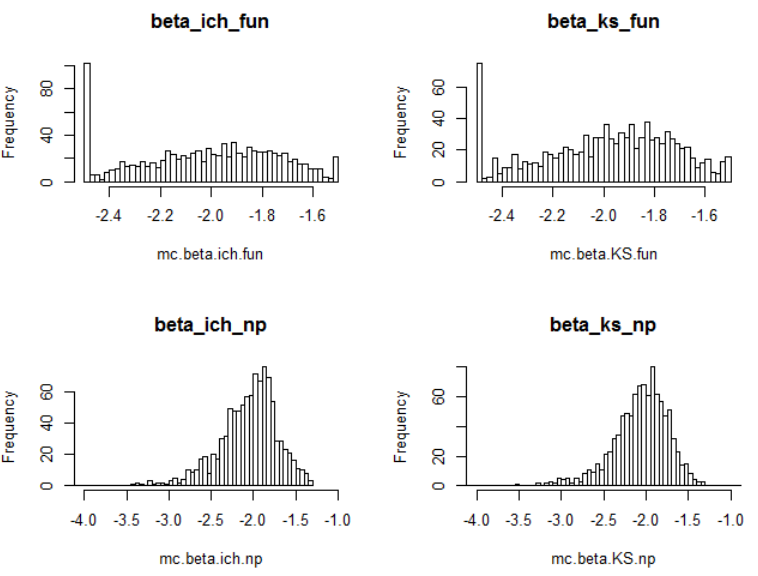
\includegraphics[width=\linewidth]{comparison_np_fun_plot.png}
 
  \label{fig:plot of estimates}
\end{figure}

A scale problem can be immediately perceived from the different ranges of x-axis, which also implies possible existence of multi-modal for $\beta$ estimates. Furthermore, due to a narrower range of the list of $\beta_2$ in Grid Search, the result of MSE is not informative on advantage of original functions either. 

To correct this mistake and make results comparable, the range of gridsearch will be adjusted to $(-4,0)$ with 0.05 space between two candidates.

\begin{table}[H]
\caption {Mean Squared Error Comparison} \label{tab:mean squared error}

(with gridsearch $(-4, 0, 81)$)

\begin{tabular}{l r r}

\toprule
\textbf{method} & \textbf{NP Package} & \textbf{Original Functions} \tabularnewline\midrule
(standard normal distribution for $x_1$, $x_2$, $\epsilon$) & &
\tabularnewline
Ichimura & 0.00363 & 0.00201 \tabularnewline
Klein and Spady & 0.00416 & 0.0000893 \tabularnewline

\bottomrule
\end{tabular}
\end{table}

\begin{figure}[h!]
  \caption{Plot of Estimates on the Same Scale}
  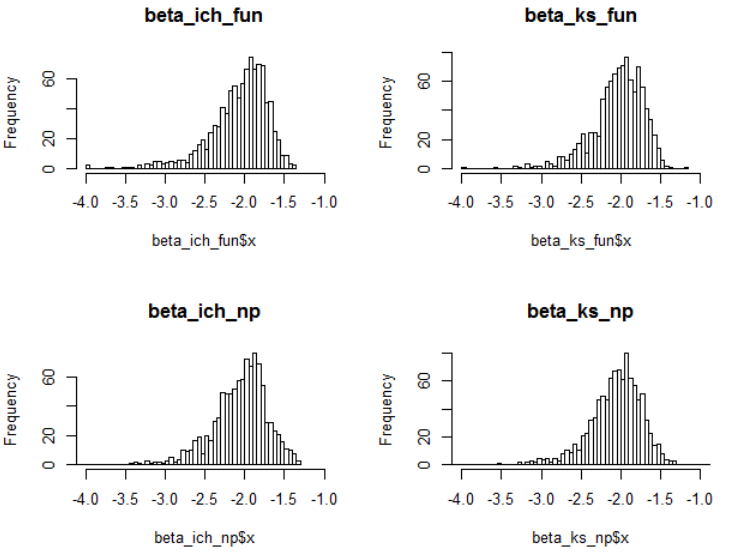
\includegraphics[width=\linewidth]{compare_done.png}
 
  \label{fig:plot of estimates on the same scale}
\end{figure}

Now we can find out that the performance of originally defined programming functions are at least as good as of NP package, and the frequency plot of both are skewed to left, implying an asymptotic feature of estimator.

\subsection{Interpretation of Results}
\label{interpretation of results}

An immediate question after observing the results in tables above is, why MSE in original functions are all significantly smaller than that calculated from the NP package?
Although it can be perceived from Figure 3 that the range of estimates obtained from NP package is wider than from original functions, i.e. the minimum of $beta\_ich\_np$ equals to $-5.079976$ whereas the minimum of $beta\_ich\_fun$ is set to be $-4$, MSE of NP package decreases but very slightly if we rule out estimates out of the range $(-4,0)$, which is still not comparable to the MSE of original functions. 

\begin{figure}[h!]
  \caption{Boxplots of Estimates}
  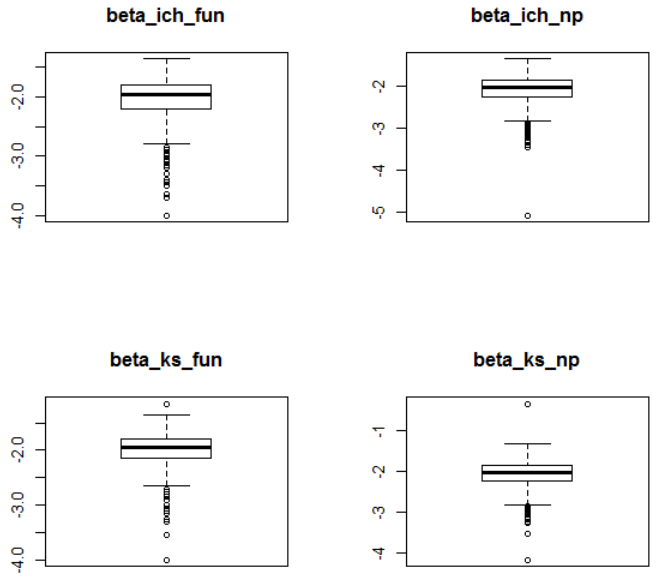
\includegraphics[width=\linewidth]{boxplot_beta.png}
 
  \label{fig:boxplots of estimates}
\end{figure}

Another thought refers to the accuracy of estimate-searching. In NP package an estimate satisfies a relative convergence tolerance of $1e-8$, which is much finer than an accuracy rate of $0.05$ defined in original functions. While it is not clear whether this difference can give rise to a higher variance of estimates of the former than the latter, the reason might exist in the optimization procedure nested in optim() function. We therefore do not go into details on this issue and will only focus on original functions.

The second question resides in an interpretation of the magnificently smaller MSE of Klein and Spady's estimates in comparison with that of Ichimura estimates when using original functions. This can be explained by the difference in efficiency between the two estimates. Notice that residuals in binary choice model only take two values depending on independent variables $x_i$ and are thus heteroskedastic by definition, the estimate in Klein and Spady's model is efficient compared to that in Ichimura's model, which requires a sensible weight function. For simplicity we stick to the `natural` weight function $w(x_i)=1$ in this paper. 

Meanwhile this relationship is reversed in the case of NP package, yet again a detailed knowledge on the NP package is required to find the real reason. 



\end{document}

